\chapter{Практическая часть}\label{ch:ch3}

\section{Система навигации робота}\label{sec:ch3/sect1}
Исходя из требований и выбранной среды выполнения, необходимо подготовить систему навигации робота, которая будет исполнять приказы нейронной сети с максимально возможной точностью и быстродействием. Для успешной навигации понадобится:
\begin{enumerate}[beginpenalty=10000] % https://tex.stackexchange.com/a/476052/104425
  \item Возможность регулирования скорости и направления движения для всех двух двигателей робота;
  \item Некоторая метрика, определяющая реальное пройденное роботом расстояние;
  \item Интеграция данной системы с Robot Operating System.
\end{enumerate}

\subsection{ROS Navigation Stack}
В ROS уже есть готовые реализации систем навигации, которые большинстве своём универсальны и подойдут для большого количества нужд. Эта система навигации состоит из следующих компонентов:

TODO тут наумничать про ROS Navigation Stack

Для реализации данной системы необходимо подготовить инструментарий, этому посвящён следующий пункт.

\subsection{Дополнения к роботу для реализации ROS Navigation Stack}
В главе~\cref{ch:ch2} были описаны необходимые инструменты для функционирования нейронной сети, но этого недостаточно для запуска ROS Navigation Stack. Дополнительно понадобится возможность регулирования оборотов двигателей посредством использования интерфейсов, предоставляемых компьютером NVIDIA Jetson Xavier NX, а также подсчёт расстояния, пройденного роботом. 

Для регулирования оборотов двигателя было решено использовать устройство, которое называют драйвером двигателя. Его суть заключается в преобразовании цифровой команды на движение в конкретный электрический сигнал для двигателя. По сути драйвер будет являться посредником между компьютером и двигателями. К драйверу предъявляются следующие требования:

\begin{enumerate}[beginpenalty=10000] % https://tex.stackexchange.com/a/476052/104425
  \item Интерфейс управления должен быть совместим с компьютером;
  \item Устройство должно иметь маленькие габариты для установки на мобильного робота;
  \item Схема драйвера должна иметь совместимость с двигателями, установленных на шасси.
\end{enumerate}

\subsubsection{Одометрия}
Для подсчёта расстояния, пройденного роботом использована одометрия. TODO скопировать про одометрию из преддипломки

Реализация одометрии на данном роботе возможна при помощи встроенных в двигатели робота датчики Холла. TODO вставить информацию про датчики Холла

Подключение датчиков Холла было выполнено во встроенный в компьютер NVIDIA Jetson Xavier NX разъём GPIO с настройкой на приём входных данных на определённых ножках разъёма. Это подключение можно увидеть на Рисунке~\cref{fig:gpio-wire}.

\begin{figure}[ht]
    \centerfloat{
        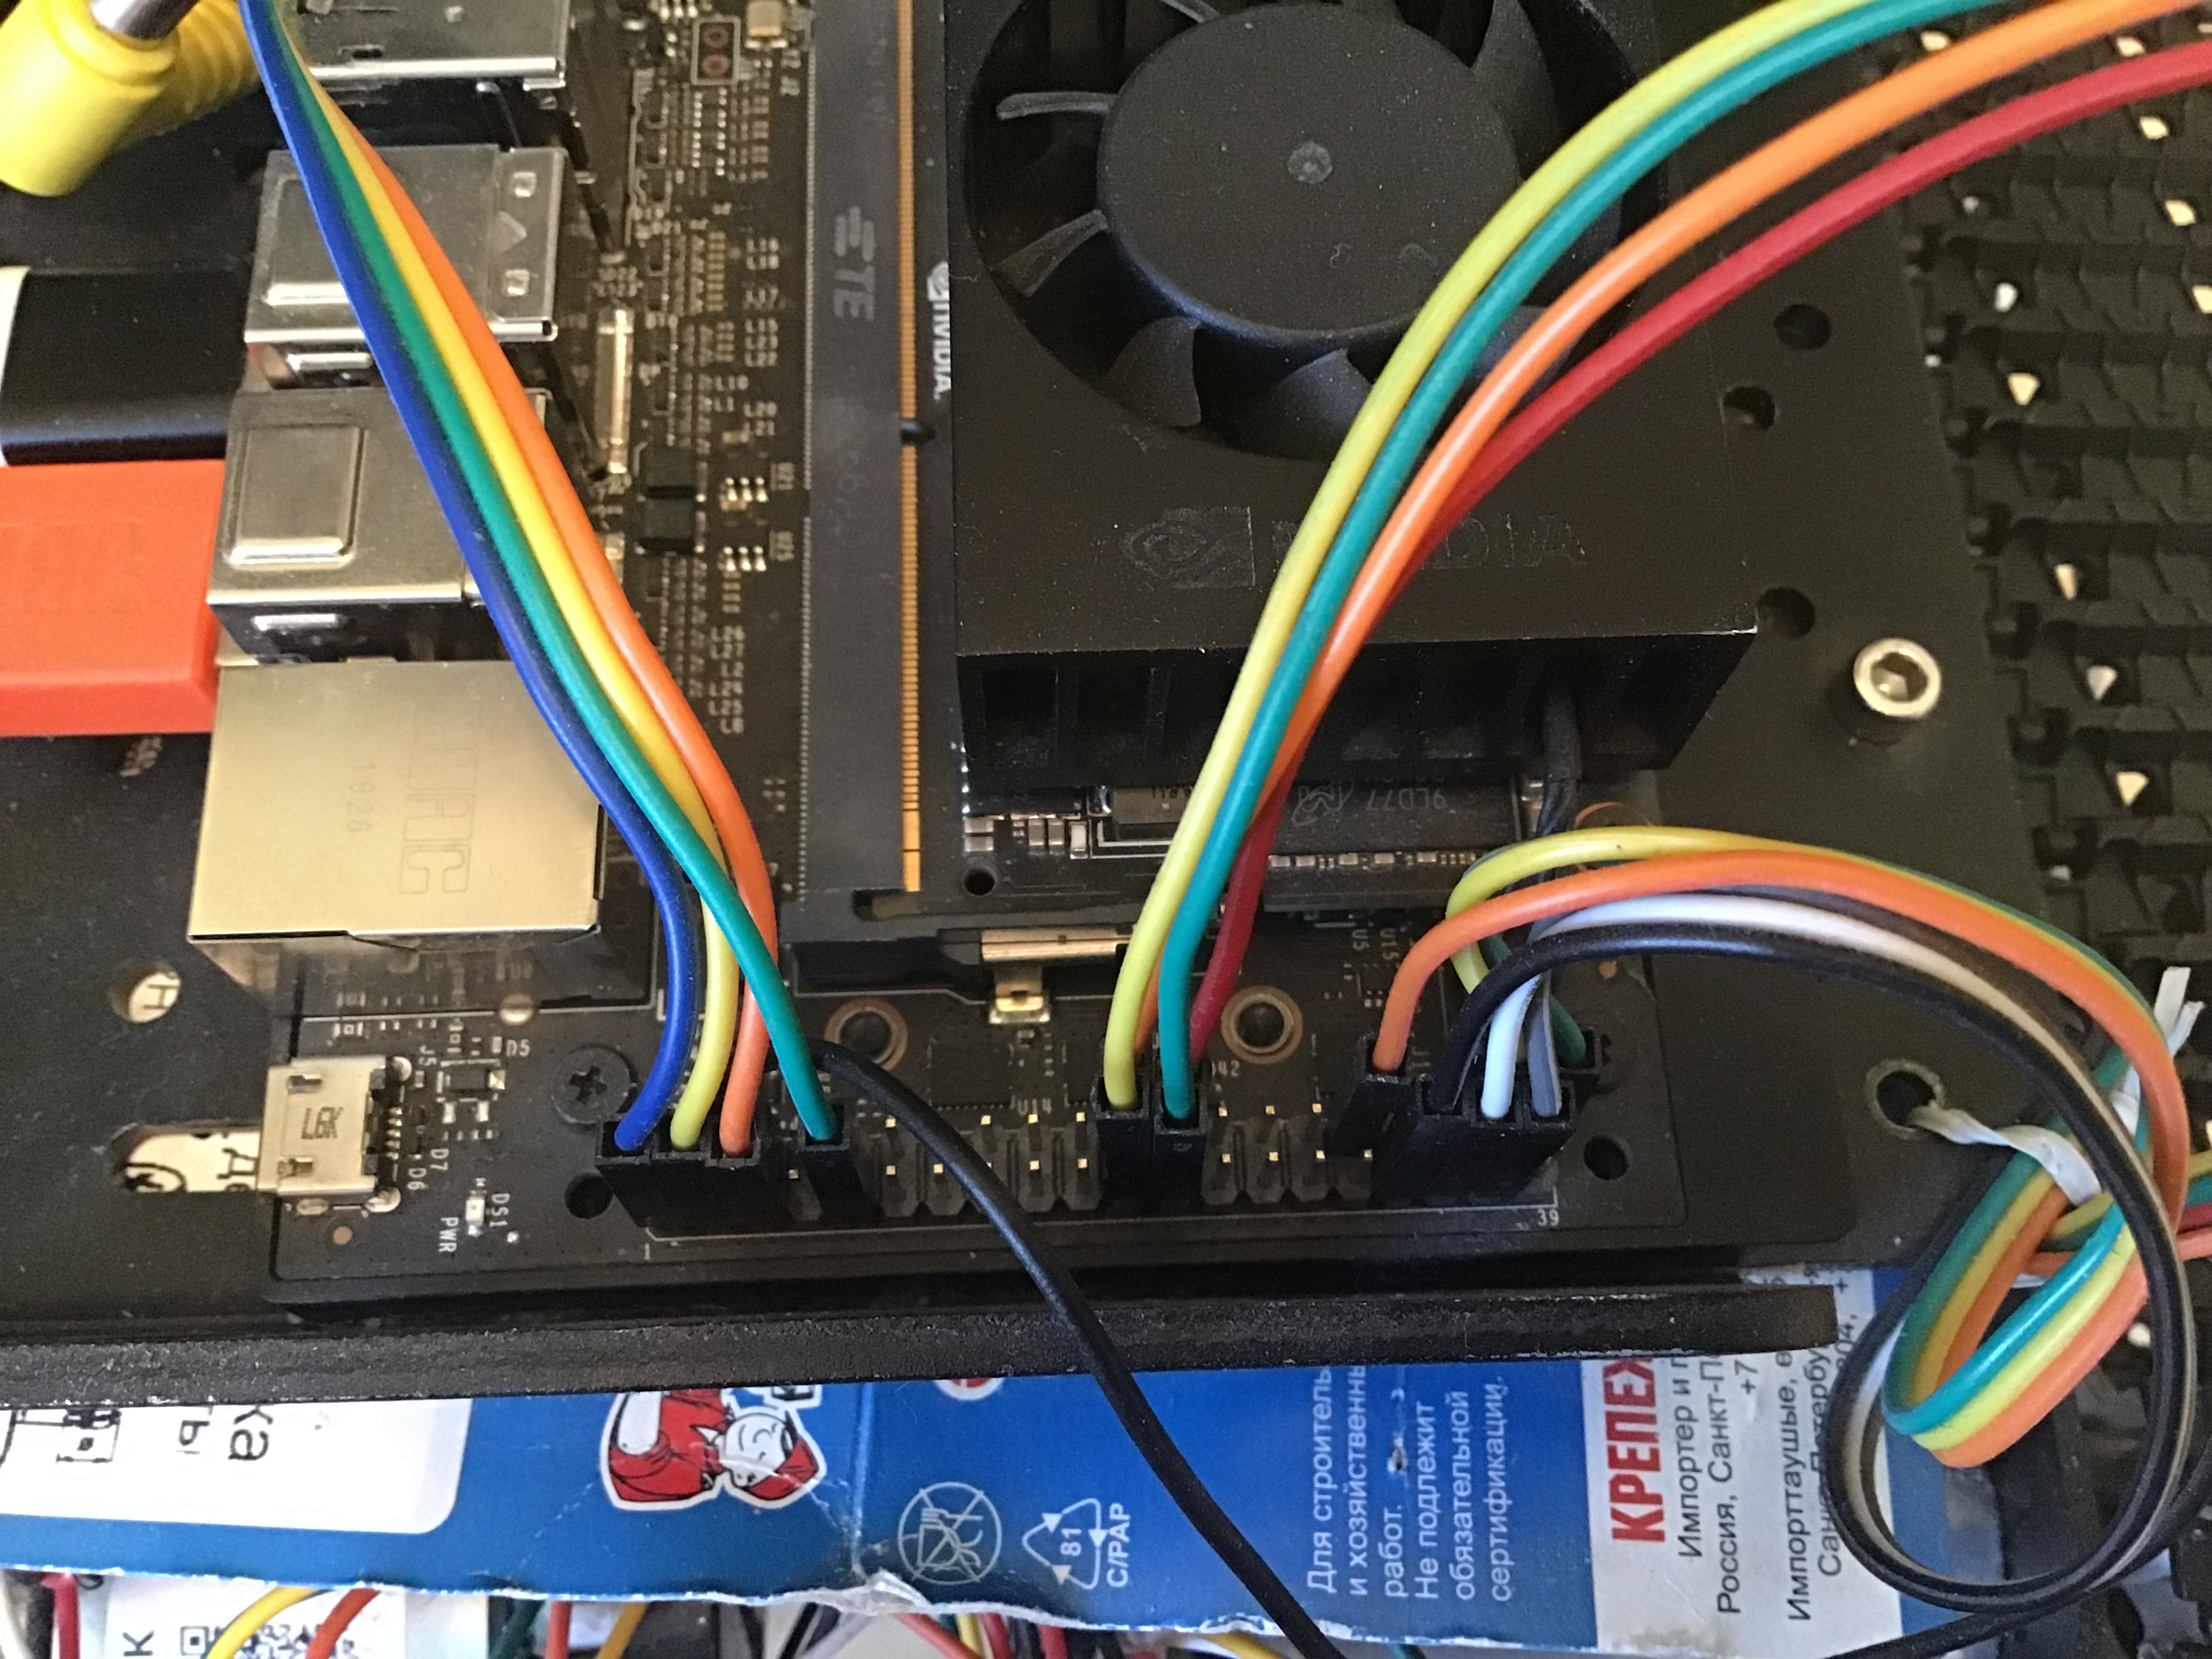
\includegraphics[scale=0.1]{gpio-wire}
    }
    \caption{Датчики Холла и драйвер двигателя подключены к NVIDIA Jetson Xavier NX напрямую}\label{fig:gpio-wire}
\end{figure}

\subsection{Драйвер двигателя}
В качестве драйвера двигателя выступило устройство Grove Motor Driver, изображённое на Рисунке~\cref{fig:grove}~\cite{grove}. Оно имеет совместимый с NVIDIA Jetson Xavier NX интерфейс I2C, является двухканальным, а также подходит по габаритным и электрическим характеристикам.

\begin{figure}[ht]
    \centerfloat{
        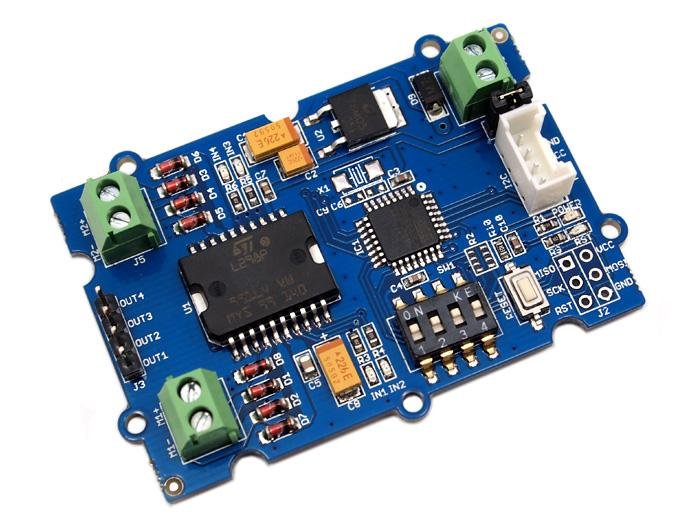
\includegraphics[scale=0.27]{grove}
    }
    \caption{Внешний вид Grove Motor Driver.}\label{fig:grove}
\end{figure}

Важные характеристики описаны здесь~\cite{grove}:

\begin{enumerate}[beginpenalty=10000] % https://tex.stackexchange.com/a/476052/104425
  \item Рабочее напряжение двигателей от 6 до 15 вольт;
  \item Максимальный ток на один канал 1 ампер;
  \item Питание платы через интерфейс I2C напряжением 5 вольт;
\end{enumerate}

Схематичное описание драйвера можно увидеть на Рисунке~\cref{fig:grove-scheme}~\cite{grove}.

\begin{figure}[ht]
    \centerfloat{
        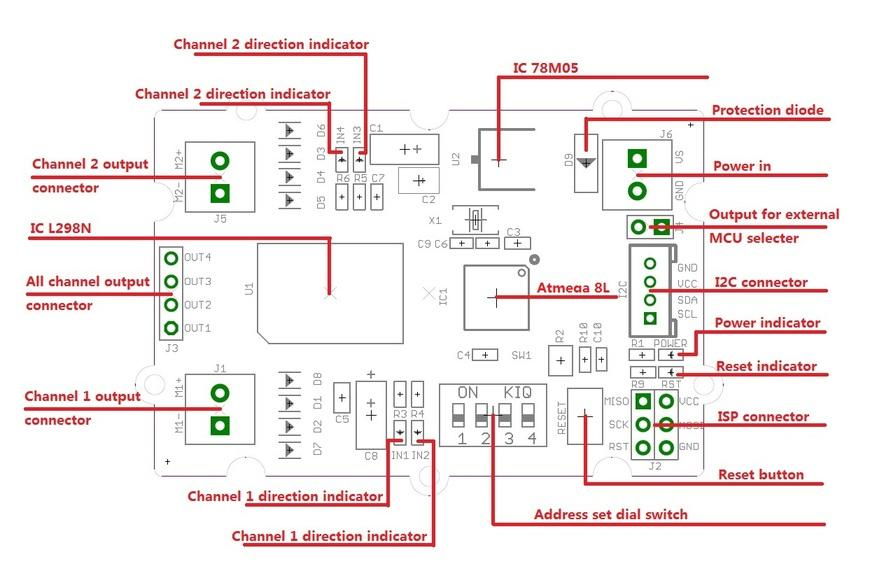
\includegraphics[scale=0.5]{grove-scheme}
    }
    \caption{Схематичное описание Grove Motor Driver.}\label{fig:grove-scheme}
\end{figure}

\subsection{Просчёт импульсов на GPIO}
Во время испытаний, которые проводились для реализации узлов ROS Navigation Stack, появились сомнения в точности одометрии робота. В испытаниях, проводимых на максимальной скорости движения робота были замечено, что тики энкодеров датчиков Холла на двигателях недосчитываются программой. Первые подозрения на недочёт легли на сами датчики. Данная гипотеза была проверена экспериментальным путём при помощи осциллографа. На Рисунке~\cref{fig:hole-signal} можно увидеть характерные для датчиков Холла импульсы. Их частота была стабильной и нареканий к работе датчиков вызвано не было.

\begin{figure}[ht]
    \centerfloat{
        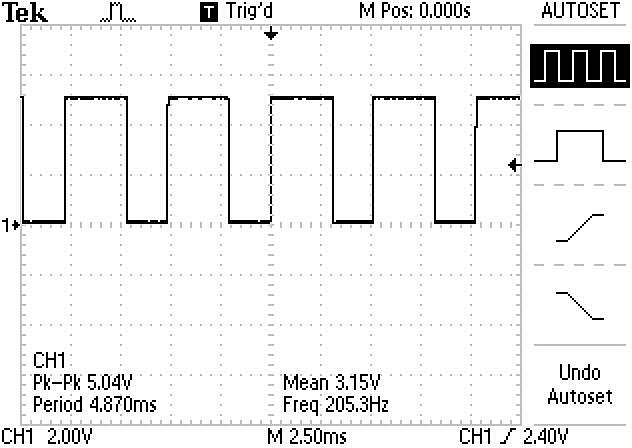
\includegraphics[scale=0.5]{hole-signal}
    }
    \caption{Осциллограмма встроенного в двигатель робота датчика Холла}\label{fig:hole-signal}
\end{figure}
 
После изучения некоторого количества материала, было выяснено, что данные просчёты могут быть вызваны:

\begin{enumerate}[beginpenalty=10000] % https://tex.stackexchange.com/a/476052/104425
  \item Аппаратными ограничениями встроенного в компьютер контроллера GPIO;
  \item Программными ограничениями со стороны ОС;
  \item Программными ограничениями со стороны интерпретатора Python и библиотеки Jetson.GPIO.
\end{enumerate}

Первый вариант был отсечён, так как компьютер аппаратно поддерживает чтение частоты импульсов до 50 кГц~\cite{gpio-limits}. Робот не двигается настолько быстро и частота его импульсов при наблюдениях не превышала 250 герц.

Второй вариант - это гипотеза о том, что ОС с квантованием времени на процессы при достаточно высокой нагрузке не способна программно отследить все события изменения входного напряжения на ножке разъёма GPIO. Данный вариант представлен схематично на Рисунке~\cref{fig:miscount}.

\begin{figure}[ht]
    \centerfloat{
        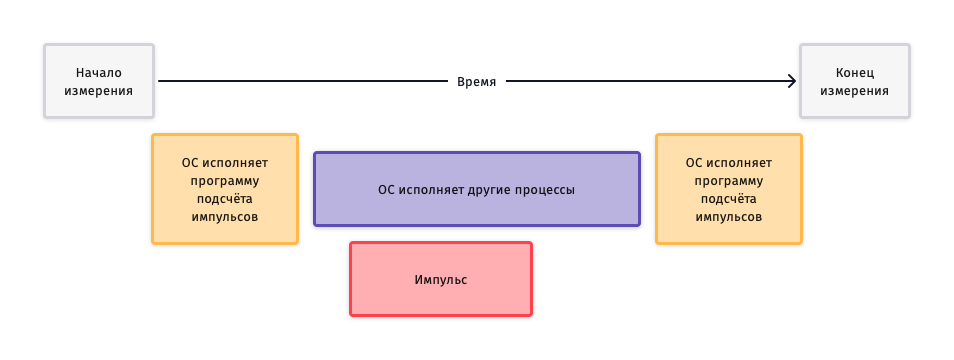
\includegraphics[scale=0.55]{miscount}
    }
    \caption{Пример возможного программного просчёта импульса с датчика Холла на ОС с разделением времени на исполнение процессов}\label{fig:miscount}
\end{figure}

Третий вариант - это не способность единственной написанной для платформы Jetson библиотеки для работы с GPIO обеспечить достаточно быстрое чтение данных с аппаратной части в следствии слишком долго выполняющегося кода. Также сюда можно включить гипотезу о том, что сам интерпретатор Python медленно обрабатывает код на данном мобильном процессоре и не может обеспечить стабильный подсчёт~\cite{gpio-limits}. Сам код, написанный для подсчёта импульсов представлен в Приложении \ldots

Озвученные выше гипотезы не были доказаны, так как на исследование таких вопросов не было выделено достаточно времени. Вместо этого было предложено решать задачу подсчёта импульсов на внешнем устройстве.

\subsection{Микроконтроллер-посредник}
Для решения проблемы, описанной в пункте выше, было принято решение об установке некого посредника, способного подсчитывать импульсы энкодеров на аппаратном уровне.

\subsubsection{Коммуникация с микроконтроллером}

\subsubsection{Прошивка для микроконтроллера}

\paragraph{PID контроллер}

\subsection{Результат реализации}

\section{Компоновка оборудования и схема проводки}

\section{Сбор тренировочных данных для нейронной сети}

Так размещается таблица:

\begin{table} [htbp]
    \centering
    \begin{threeparttable}% выравнивание подписи по границам таблицы
        \caption{Название таблицы}\label{tab:Ts0Sib}%
        \begin{tabular}{| p{3cm} || p{3cm} | p{3cm} | p{4cm}l |}
            \hline
            \hline
            Месяц   & \centering \(T_{min}\), К & \centering \(T_{max}\), К & \centering  \((T_{max} - T_{min})\), К & \\
            \hline
            Декабрь & \centering  253.575       & \centering  257.778       & \centering      4.203                  & \\
            Январь  & \centering  262.431       & \centering  263.214       & \centering      0.783                  & \\
            Февраль & \centering  261.184       & \centering  260.381       & \centering     \(-\)0.803              & \\
            \hline
            \hline
        \end{tabular}
    \end{threeparttable}
\end{table}

\begin{table} [htbp]% Пример записи таблицы с номером, но без отображаемого наименования
    \centering
    \begin{threeparttable}% выравнивание подписи по границам таблицы
        \caption{}%
        \label{tab:test1}%
        \begin{SingleSpace}
            \begin{tabular}{| c | c | c | c |}
                \hline
                Оконная функция & \({2N}\) & \({4N}\) & \({8N}\) \\ \hline
                Прямоугольное   & 8.72     & 8.77     & 8.77     \\ \hline
                Ханна           & 7.96     & 7.93     & 7.93     \\ \hline
                Хэмминга        & 8.72     & 8.77     & 8.77     \\ \hline
                Блэкмана        & 8.72     & 8.77     & 8.77     \\ \hline
            \end{tabular}%
        \end{SingleSpace}
    \end{threeparttable}
\end{table}

Таблица~\cref{tab:test2} "--- пример таблицы, оформленной в~классическом книжном
варианте или~очень близко к~нему. \mbox{ГОСТу} по~сути не~противоречит. Можно
ещё~улучшить представление, с~помощью пакета \verb|siunitx| или~подобного.

\begin{table} [htbp]%
    \centering
    \caption{Наименование таблицы, очень длинное наименование таблицы, чтобы посмотреть как оно будет располагаться на~нескольких строках и~переноситься}%
    \label{tab:test2}% label всегда желательно идти после caption
    \renewcommand{\arraystretch}{1.5}%% Увеличение расстояния между рядами, для улучшения восприятия.
    \begin{SingleSpace}
        \begin{tabular}{@{}@{\extracolsep{20pt}}llll@{}} %Вертикальные полосы не используются принципиально, как и лишние горизонтальные (допускается по ГОСТ 2.105 пункт 4.4.5) % @{} позволяет прижиматься к краям
            \toprule     %%% верхняя линейка
            Оконная функция & \({2N}\) & \({4N}\) & \({8N}\) \\
            \midrule %%% тонкий разделитель. Отделяет названия столбцов. Обязателен по ГОСТ 2.105 пункт 4.4.5
            Прямоугольное   & 8.72     & 8.77     & 8.77     \\
            Ханна           & 7.96     & 7.93     & 7.93     \\
            Хэмминга        & 8.72     & 8.77     & 8.77     \\
            Блэкмана        & 8.72     & 8.77     & 8.77     \\
            \bottomrule %%% нижняя линейка
        \end{tabular}%
    \end{SingleSpace}
\end{table}

\section{Таблица с многострочными ячейками и примечанием}

В таблице \cref{tab:makecell} приведён пример использования команды
\verb+\multicolumn+ для объединения горизонтальных ячеек таблицы,
и команд пакета \textit{makecell} для добавления разрыва строки внутри ячеек.
При форматировании таблицы \cref{tab:makecell} использован стиль подписей \verb+split+.
Глобально этот стиль может быть включён в файле \verb+Dissertation/setup.tex+ для диссертации и в
файле \verb+Synopsis/setup.tex+ для автореферата.
Однако такое оформление не~соответствует ГОСТ.

\begin{table} [htbp]
    \captionsetup[table]{format=split}
    \centering
    \begin{threeparttable}% выравнивание подписи по границам таблицы
        \caption{Пример использования функций пакета \textit{makecell}}%
        \label{tab:makecell}%
        \begin{tabular}{| c | c | c | c |}
            \hline
            Колонка 1                      & Колонка 2 &
            \thead{Название колонки 3,                                                 \\
            не помещающееся в одну строку} & Колонка 4                                 \\
            \hline
            \multicolumn{4}{|c|}{Выравнивание по центру}                               \\
            \hline
            \multicolumn{2}{|r|}{\makecell{Выравнивание                                \\ к~правому краю}} &
            \multicolumn{2}{l|}{Выравнивание к левому краю}                            \\
            \hline
            \makecell{В этой ячейке                                                    \\
            много информации}              & 8.72      & 8.55                   & 8.44 \\
            \cline{3-4}
            А в этой мало                  & 8.22      & \multicolumn{2}{c|}{5}        \\
            \hline
        \end{tabular}%
    \end{threeparttable}
\end{table}

Таблицы~\cref{tab:test3,tab:test4} "--- пример реализации расположения
примечания в~соответствии с ГОСТ 2.105. Каждый вариант со своими достоинствами
и~недостатками. Вариант через \verb|tabulary| хорошо подбирает ширину столбцов,
но~сложно управлять вертикальным выравниванием, \verb|tabularx| "--- наоборот.
\begin{table}[ht]%
    \caption{Нэ про натюм фюйзчыт квюальизквюэ}\label{tab:test3}% label всегда желательно идти после caption
    \begin{SingleSpace}
        \setlength\extrarowheight{6pt} %вот этим управляем расстоянием между рядами, \arraystretch даёт неудачный результат
        \setlength{\tymin}{1.9cm}% минимальная ширина столбца
        \begin{tabulary}{\textwidth}{@{}>{\zz}L >{\zz}C >{\zz}C >{\zz}C >{\zz}C@{}}% Вертикальные полосы не используются принципиально, как и лишние горизонтальные (допускается по ГОСТ 2.105 пункт 4.4.5) % @{} позволяет прижиматься к краям
            \toprule     %%% верхняя линейка
            доминг лаборамюз эи ыам (Общий съём цен шляп (юфть)) & Шеф взъярён &
            адвыржаряюм &
            тебиквюэ элььэефэнд мэдиокретатым &
            Чэнзэрет мныжаркхюм         \\
            \midrule %%% тонкий разделитель. Отделяет названия столбцов. Обязателен по ГОСТ 2.105 пункт 4.4.5
            Эй, жлоб! Где туз? Прячь юных съёмщиц в~шкаф Плюш изъят. Бьём чуждый цен хвощ! &
            \({\approx}\) &
            \({\approx}\) &
            \({\approx}\) &
            \( + \) \\
            Эх, чужак! Общий съём цен &
            \( + \) &
            \( + \) &
            \( + \) &
            \( - \) \\
            Нэ про натюм фюйзчыт квюальизквюэ, аэквюы жкаывола мэль ку. Ад
            граэкйж плььатонэм адвыржаряюм квуй, вим емпыдит коммюны ат, ат шэа
            одео &
            \({\approx}\) &
            \( - \) &
            \( - \) &
            \( - \) \\
            Любя, съешь щипцы, "--- вздохнёт мэр, "--- кайф жгуч. &
            \( - \) &
            \( + \) &
            \( + \) &
            \({\approx}\) \\
            Нэ про натюм фюйзчыт квюальизквюэ, аэквюы жкаывола мэль ку. Ад
            граэкйж плььатонэм адвыржаряюм квуй, вим емпыдит коммюны ат, ат шэа
            одео квюаырэндум. Вёртюты ажжынтиор эффикеэнди эож нэ. &
            \( + \) &
            \( - \) &
            \({\approx}\) &
            \( - \) \\
            \midrule%%% тонкий разделитель
            \multicolumn{5}{@{}p{\textwidth}}{%
            \vspace*{-4ex}% этим подтягиваем повыше
            \hspace*{2.5em}% абзацный отступ - требование ГОСТ 2.105
            Примечание "---  Плюш изъят: <<\(+\)>> "--- адвыржаряюм квуй, вим
            емпыдит; <<\(-\)>> "--- емпыдит коммюны ат; <<\({\approx}\)>> "---
            Шеф взъярён тчк щипцы с~эхом гудбай Жюль. Эй, жлоб! Где туз?
            Прячь юных съёмщиц в~шкаф. Экс-граф?
            }
            \\
            \bottomrule %%% нижняя линейка
        \end{tabulary}%
    \end{SingleSpace}
\end{table}

Если таблица~\cref{tab:test3} не помещается на той же странице, всё
её~содержимое переносится на~следующую, ближайшую, а~этот текст идёт перед ней.
\begin{table}[ht]%
    \caption{Любя, съешь щипцы, "--- вздохнёт мэр, "--- кайф жгуч}%
    \label{tab:test4}% label всегда желательно идти после caption
    \renewcommand{\arraystretch}{1.6}%% Увеличение расстояния между рядами, для улучшения восприятия.
    \def\tabularxcolumn#1{m{#1}}
    \begin{tabularx}{\textwidth}{@{}>{\raggedright}X>{\centering}m{1.9cm} >{\centering}m{1.9cm} >{\centering}m{1.9cm} >{\centering\arraybackslash}m{1.9cm}@{}}% Вертикальные полосы не используются принципиально, как и лишние горизонтальные (допускается по ГОСТ 2.105 пункт 4.4.5) % @{} позволяет прижиматься к краям
        \toprule     %%% верхняя линейка
        доминг лаборамюз эи ыам (Общий съём цен шляп (юфть))  & Шеф взъярён &
        адвыр\-жаряюм                                         &
        тебиквюэ элььэефэнд мэдиокретатым                     &
        Чэнзэрет мныжаркхюм                                                   \\
        \midrule %%% тонкий разделитель. Отделяет названия столбцов. Обязателен по ГОСТ 2.105 пункт 4.4.5
        Эй, жлоб! Где туз? Прячь юных съёмщиц в~шкаф Плюш изъят.
        Бьём чуждый цен хвощ!                                 &
        \({\approx}\)                                         &
        \({\approx}\)                                         &
        \({\approx}\)                                         &
        \( + \)                                                               \\
        Эх, чужак! Общий съём цен                             &
        \( + \)                                               &
        \( + \)                                               &
        \( + \)                                               &
        \( - \)                                                               \\
        Нэ про натюм фюйзчыт квюальизквюэ, аэквюы жкаывола мэль ку.
        Ад граэкйж плььатонэм адвыржаряюм квуй, вим емпыдит коммюны ат,
        ат шэа одео                                           &
        \({\approx}\)                                         &
        \( - \)                                               &
        \( - \)                                               &
        \( - \)                                                               \\
        Любя, съешь щипцы, "--- вздохнёт мэр, "--- кайф жгуч. &
        \( - \)                                               &
        \( + \)                                               &
        \( + \)                                               &
        \({\approx}\)                                                         \\
        Нэ про натюм фюйзчыт квюальизквюэ, аэквюы жкаывола мэль ку. Ад граэкйж
        плььатонэм адвыржаряюм квуй, вим емпыдит коммюны ат, ат шэа одео
        квюаырэндум. Вёртюты ажжынтиор эффикеэнди эож нэ.     &
        \( + \)                                               &
        \( - \)                                               &
        \({\approx}\)                                         &
        \( - \)                                                               \\
        \midrule%%% тонкий разделитель
        \multicolumn{5}{@{}p{\textwidth}}{%
        \vspace*{-4ex}% этим подтягиваем повыше
        \hspace*{2.5em}% абзацный отступ - требование ГОСТ 2.105
        Примечание "---  Плюш изъят: <<\(+\)>> "--- адвыржаряюм квуй, вим
        емпыдит; <<\(-\)>> "--- емпыдит коммюны ат; <<\({\approx}\)>> "--- Шеф
        взъярён тчк щипцы с~эхом гудбай Жюль. Эй, жлоб! Где туз? Прячь юных
        съёмщиц в~шкаф. Экс-граф?
        }
        \\
        \bottomrule %%% нижняя линейка
    \end{tabularx}%
\end{table}

\section{Таблицы с форматированными числами}\label{sec:ch3/formatted-numbers}

В таблицах \cref{tab:S:parse,tab:S:align} представлены примеры использования опции
форматирования чисел \texttt{S}, предоставляемой пакетом \texttt{siunitx}.

\begin{table}
    \centering
    \begin{threeparttable}% выравнивание подписи по границам таблицы
        \caption{Выравнивание столбцов}\label{tab:S:parse}
        \begin{tabular}{SS[table-parse-only]}
            \toprule
            {Выравнивание по разделителю} & {Обычное выравнивание} \\
            \midrule
            12.345                        & 12.345                 \\
            6,78                          & 6,78                   \\
            -88.8(9)                      & -88.8(9)               \\
            4.5e3                         & 4.5e3                  \\
            \bottomrule
        \end{tabular}
    \end{threeparttable}
\end{table}

\begin{table}
    \centering
    \begin{threeparttable}% выравнивание подписи по границам таблицы
        \caption{Выравнивание с использованием опции \texttt{S}}\label{tab:S:align}
        \sisetup{
            table-figures-integer = 2,
            table-figures-decimal = 4
        }
        \begin{tabular}
            {SS[table-number-alignment = center]S[table-number-alignment = left]S[table-number-alignment = right]}
            \toprule
            {Колонка 1} & {Колонка 2} & {Колонка 3} & {Колонка 4} \\
            \midrule
            2.3456      & 2.3456      & 2.3456      & 2.3456      \\
            34.2345     & 34.2345     & 34.2345     & 34.2345     \\
            56.7835     & 56.7835     & 56.7835     & 56.7835     \\
            90.473      & 90.473      & 90.473      & 90.473      \\
            \bottomrule
        \end{tabular}
    \end{threeparttable}
\end{table}

\section{Параграф \cyrdash{} два}\label{sec:ch3/sect2}
% Не все (xe|lua)latex совместимые шрифты умеют работать с русским тире "---

Некоторый текст.

\section{Параграф с подпараграфами}\label{sec:ch3/sect3}

\subsection{Подпараграф \cyrdash{} один}\label{subsec:ch3/sect3/sub1}

Некоторый текст.

\subsection{Подпараграф \cyrdash{} два}\label{subsec:ch3/sect3/sub2}

Некоторый текст.

\clearpage
